\begin{chapquote}{Someone said this}
``This was said.''
\end{chapquote}

\section{Deciphering Practice: 
\\Substitution \& Vigen\`ere Ciphers}

\underline{Warm Up:}\\
The solution to the Substitution Cipher and the great advice about problem solving was: "The best way to learn math is to do lots of problems:  after all, that's what math is!  If you want to get good at rock climbing, it doesn't make sense to only sit down and read a bunch of books on rock climbing. You eventually have to get on the rock and try some of the techniques you read about."

The \defi{Vigen\`ere Cipher} is a \defi{polyalphabetic cipher} meaning that it uses 26 cipher alphabets to encrypt a message.
The steps to encipher a message are:
\begin{enumerate}
\item Draw the Vigen\`ere Square, where each row represents a \defi{Caesar Shift} row, but beginning one letter later.So row 1 is a \defi{Caesar Shift} of 1, row 2 is a Caesar shift of 2...etc.  See Figure~\ref{fig:VigSquare}
\item Use all the rows to encipher the message
\end{enumerate}


\begin{figure}
\centering
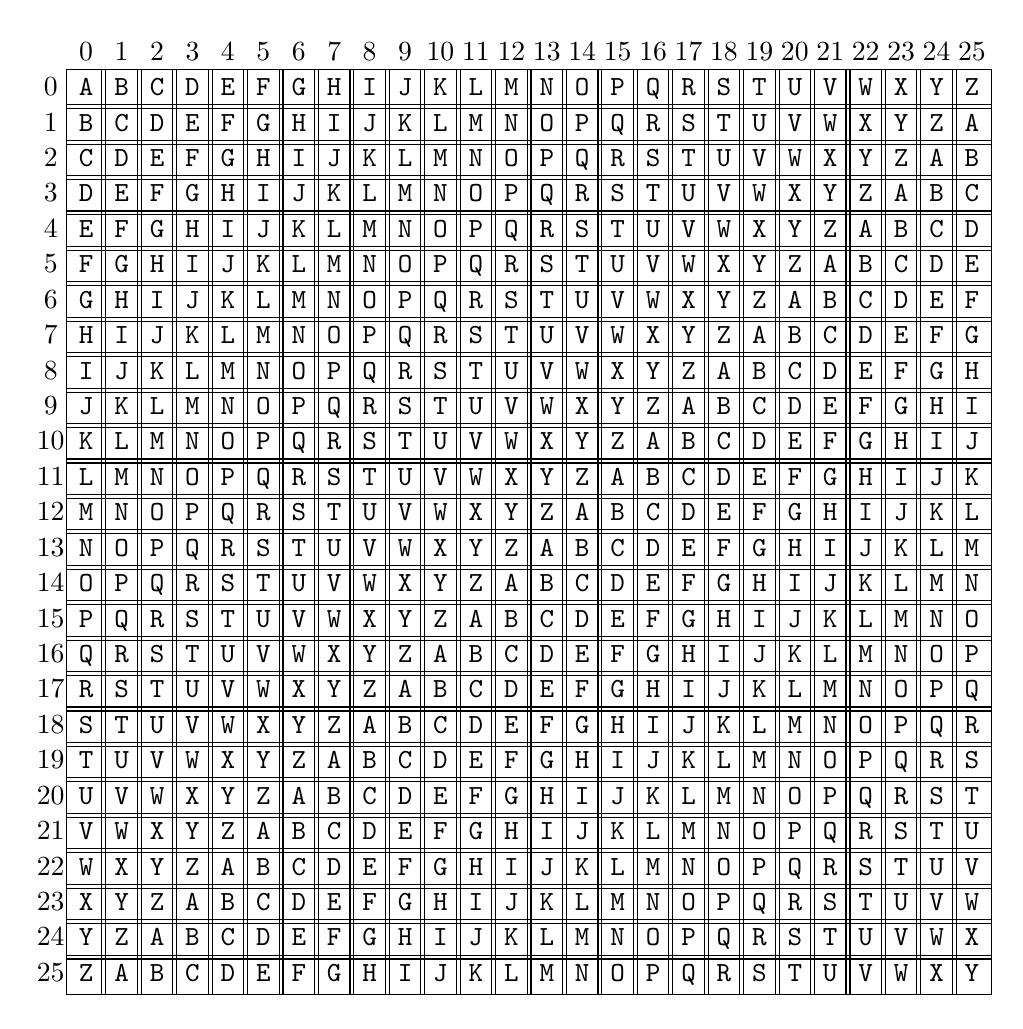
\begin{tikzpicture}[scale=.9]
\foreach \i in {0,...,25} {
  \foreach \j in {0,...,25} {
    \edef\k{\ifnum\numexpr\i+\j\relax>25
        \the\numexpr\i+\j-26\relax
      \else
        \the\numexpr\i+\j\relax
      \fi}
  \node[draw,minimum size=0.5cm,inner sep=0pt]
    at (\i*0.5,-\j*0.5) {\strut{\tt \symbol{\numexpr`A+\k\relax}}};
  }
  \node at (-0.5,-\i*0.5) {\strut\i};
  \node at (\i*0.5,0.5)   {\strut\i};
}
\end{tikzpicture}
\caption{A Vigen\`ere square.}
\label{fig:VigSquare}
\end{figure}

The steps to unscramble the message are:
\begin{enumerate}
\item Having established an agreed system for row switching, use the \defi{keyword} that is repeated over the ciphertext.  
\item The row in the \defi{Vigen\`ere Square} that begins with the letter of the keyword that is above the first letter of the ciphertext is the one you use to decipher the first letter.  The row in the \defi{Vigen\`ere Square} that begins with the letter of the keyword that is above the second letter of the ciphertext is the one you use to decipher the second letter.  This continues until the message is over, as the keyword is repeated multiple times over the ciphertext.
\end{enumerate}

\underline{Key aspects of the Vigen\`ere Cipher:}
\begin{enumerate}
\item Frequency analysis cannot handle this cipher as accurately as we would like because the ciphertext letters that repeat don't necessarily represent the same plaintext letters and vice versa
\item There are a lot of options for a keyword, making the message more secure
\end{enumerate}

\underline{Tips for deciphering Vigen\`ere Ciphers:}
\begin{enumerate}
\item Look for repeated strings.
\item Count the spaces between each of the individual strings.
\item Compile a list of all the factors of the space numbers and look for a common one among them.  This is in order to determine the length of the codeword used to encipher the message.
\item Once the length of the codeword has been determined, split the enciphered text into groups according to the length of the codeword.  Thus, if the codeword was 3 letters long, you would have L1, L2, L3, where L1 represents, beginning at the first letter, every third letter (that was enciphered with one particular cipher alphabet), L2 represents, beginning at the second letter, every third letter (enchiphered with a different cipher alphabet) and so on.
\item Perform frequency analysis on each of the indiviual groups created.
\end{enumerate}

\underline{Pros of Vigen\`ere Ciphers:}
\begin{itemize}
\item Lots of possible keys for encryptions
\item Lots of alphabets (Polyalphabetic): Many to many function
\item Fools Frequency Analysis
\item Requires counting (You can try to avoid repeated strings)
\item (In the 1800's) Lack of technology at the time
\item (In the 1800's) Length of message could be the keyword.  The upperbound would then be $26^\text{(length of the message)}$
\end{itemize}

\underline{Cons of Vigen\`ere Cipher:}
\begin{itemize}
\item Lots of alphabets, thus slower enciphering and deciphering
\item Requires counting
\item Can be cracked with math and Frequency Analysis
\item Still requires sender/reciever to know keyword
\item Caesar shifts are used, so once you find one letter, you know the whole alphabet
\item (In the 1800's) Mechanization [computers]
\end{itemize}

\section{Number Theory and Counting}

Goal: Find the number of k-element subests of an n-element set.

\begin{example} My friends and I have 55 cats. We want to enter 3 into the "Loveliest Cat" competition. How many distinct ways can I do it? \\

$$Solution: \frac{55 \times 54 \times 53}{3!} = \frac{55!}{(55-3)!3!} = \binom{55}{3} = _{55}\mathrm{C}_{3}$$\\

Note: Just $55 \times 54 \times 53 = 157,410$ is NOT RIGHT! This method implies an order to the selection of cats and overcounts by $6 = 3!$ ways.\\ \\
In general, "n choose k" can be written as: $$ \binom{n}{k} = \frac{n!}{(n-k)!k!}$$
\end{example}

\begin{theorem} (Binomial Theorem)\\
$$ (x + y)^{n} = \sum_
{k=0}^{n}
{\binom{n}{k}} x^{n-k} y^{k}
$$\end{theorem}

\begin{example}
Let $n=3$.

\begin{align*}
(x + y)^3 &= \binom{3}{0}x^{3}y^{0} + \binom{3}{1}x^{2}y^{1} + \binom{3}{2}x^{1}y^{2} + \binom{3}{3}x^{0}y^{3}\\
&= 1x^{3}y^{0} + 3x^{2}y^{1} + 3x^{1}y^{2} + 1x^{0}y^{3}\\ 
&= x^{3} + 3x^{2}y + 3xy^{2} + y^{3}
\end{align*}
\end{example}


\begin{proof}
Let ${0}\leq{k}\leq{n}$. Consider the coefficient of $x^{n-k}y^{k}$. Every monomial has $n$ spots, which can each be an $x$ or a $y$. Since $x$ has exponent $n-k$, then you can choose $n-k$ spots to place $x$, (commuting after). Then the $y$'s fill in the remaining spots. Since I am looking for $n-k$ element subsets of the set of $n$ spots, then the coeffiecient is: 
$$\binom{n}{n-k} = \frac{n!}{(n-(n-k))!(n-k)!} = \frac{n!}{k!(n-k)!} = \binom{n}{k}$$
\end{proof}

\begin{proposition} From the above proof:\\
$$\binom{n}{n-k} = \binom{n}{k}$$\end{proposition}

\section{Square Numbers}

Recall from previous math classes that some examples of 'square' numbers are: $1, 4, 9, 16, 25, ...$ 
%%Look in "Resources" -->"images" folder for a visual dot picture%%
\\\\The definition was historically that $n$ is a square number if $n$ dots can be evenly arranged to form a square; see Figure~\ref{fig:squares}.

\begin{figure}[!ht]
\centering
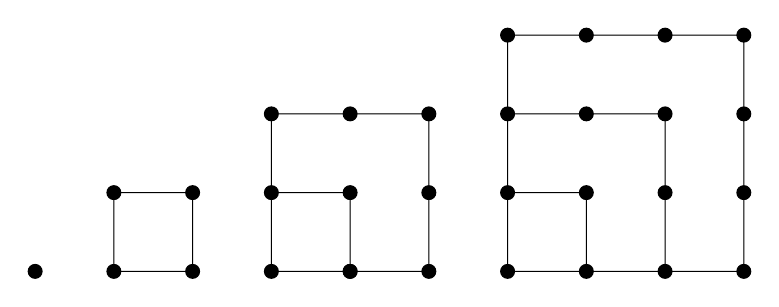
\begin{tikzpicture}
\draw[fill=black] (0,0) circle (.25em);
\draw[fill=black] (1,0) circle (.25em) -- (1,1) circle (.25em) -- (2,1) circle (.25em) -- (2,0) circle (.25em) -- (1,0); 
\draw[fill=black] (3,0) circle (.25em) -- (3,1) circle (.25em) -- (4,1) circle (.25em) -- (4,0) circle (.25em) -- (3,0);
\draw[fill=black] (3,1) -- (3,2) circle (.25em) -- (4,2) circle (.25em) -- (5,2) circle (.25em) -- (5,1) circle (.25em) -- (5,0) circle (.25em) -- (4,0) circle (.25em);
\draw[fill=black] (6,0) circle (.25em) -- (6,3) circle (.25em)-- (9,3) circle (.25em) -- (9,0) circle (.25em) -- (6,0) (7,3) circle (.25em) (8,3) circle (.25em) (9,2) circle (.25em) (9,1) circle (.25em);
\draw[fill=black] (6,2) circle (.25em) -- (8,2) circle (.25em) -- (8,0) circle (.25em) (7,2) circle (.25em) (8,1) circle (.25em);
\draw[fill=black] (6,1) circle (.25em) -- (7,1) circle (.25em) -- (7,0) circle (.25em);
\end{tikzpicture}
\caption{The definition of a square number was originally geometric.  That is, $n$ was said to be a square number if $n$ dots could be evenly arranged to form a square.  Observe, $1^{2} = 1$, $2^{2} = 1 + 3$, $3^{2} = 1 + 3 + 5$, and $4^{2} = 1 + 3 + 5 + 9$.  This observation is formalized in Proposition~\ref{prop:squares}.}\label{fig:squares}
\end{figure}

\begin{proposition}\label{prop:squares} For all positive integers $n$,  $$n^{2} =\sum_{k=0}^{n-1}{(2k+1)}.$$
\end{proposition}

\section{Diophantine Equations} % Kat

\begin{theorem}[Fermat's Last Theorem] For $n \geq 3$, $$x^n + y^n = z^n$$ has no nontrivial integer solutions.
\end{theorem}

Fermat's Last Theorem was not proven until 1994 by Andrew Wiles using the theory of elliptic curves. In this class, we will not show the proof but we will show examples. Fermat's Last Theorem will help us understand diophantine equations.


\begin{definition}
A \defi{linear diophantine equation} has the form 
\[
a_1 x_1 + a_2 x_2 + \cdots + a_n x_n = c,
\]
where $a_1,\ldots,a_n, c \in \ZZ$ and $x_1,\ldots,x_n$ are unknowns.
\end{definition}

We can write this equation in  matrix form, using matrix multiplication:
$$\begin{bmatrix}
a_1 & a_2 & \cdots & a_n
\end{bmatrix}
\begin{bmatrix}
x_1 \\
x_2 \\
\vdots\\
x_n
\end{bmatrix}
=
\begin{bmatrix}
c
\end{bmatrix}
= c.$$
Similar to matrix equations, we could have a system of linear diophantine equations whose integer solution would be a set of assignments $$x_1 = s_1, \, x_2 = s_2, \, ... \, x_n = s_n \in \ZZ.$$

\begin{theorem}\label{thm:diophantine}
Let $a, b, n, \in \ZZ$. Consider the equation $ax + by = n$. The following are true:
\begin{enumerate}
\item The equation has an integer solution if and only if $d = gcd(a,b)$ divides $n$.
\item If $(x_0,y_0)$ is a particular integer solution, then every solution takes the form \[x = x_0 + un \quad \text{and} \quad y = y_0 - vn\] for any $n \in \ZZ$, where $du = b$ and $dv = a$. 
\end{enumerate}
\end{theorem}
Before proving this theorem, let's derive number 2. Consider the example $3x + 5y = 1$. Using the Euclidean Algorithm, we can determine the greatest common denominator of 3 and 5:
\begin{align}
5 &= 3 \cdot 1 + 2 \label{eq:EEA1}\\
3 &= 2 \cdot 1 + 1 \label{eq:EEA2}\\
2 &= 1 \cdot 2 + 0 \notag
\end{align}
Using these equations, we can apply the Extended Euclidean Algorithm to find $x$ and $y$. As we go through this process, we remember to keep 3s and 5s sacred by not combining them with any other numbers. We start by rewriting Equation~\eqref{eq:EEA1} in terms of 2 and the Equation~\eqref{eq:EEA2} in terms of 1: 
\begin{align}
2 &= 5 - 3 \cdot 1 \label{eq:EEA4}\\
1 &= 3 - 2 \cdot 1. \label{eq:EEA5} 
\end{align}
Next, we can substitute for 2 in Equation~\eqref{eq:EEA5} using Equation~\eqref{eq:EEA4}:
\begin{align}
1 &= 3 - (5 - 3 \cdot 1) \cdot 1. \\
  &= 3 - 5 + 3 \\ 
  &= 2 \cdot 3 - 5
\end{align}
Therefore, $x=2$ and $y=-1$. Our Extended Euclidean Algorithm involves back-substituting the equations found using the Euclidean Algorithm until we work out way up to the first equation.

We can also find other solutions for $x$ and $y$ such as $x = -3$ and $y = 2$. By examining these solutions for $x$ and $y$, we can conclude that they are related in the following way: $x = 2 + 5n$ and $y = -1 - 3n$. From this result, we can derive number 2 in Theorem~\ref{thm:diophantine}